% ---------------------------------------------------------------------------
% Author guideline and sample document for EG publication using LaTeX2e input
% D.Fellner, v1.13, Jul 31, 2008

\documentclass{egpubl}
\usepackage{eg2016}

% --- for  Annual CONFERENCE
% \ConferenceSubmission   % uncomment for Conference submission
\ConferencePaper        % uncomment for (final) Conference Paper
% \STAR                   % uncomment for STAR contribution
% \Tutorial               % uncomment for Tutorial contribution
% \ShortPresentation      % uncomment for (final) Short Conference Presentation
% \Areas                  % uncomment for Areas contribution
% \MedicalPrize           % uncomment for Medical Prize contribution
% \Education              % uncomment for Education contribution
%
% --- for  CGF Journal
% \JournalSubmission    % uncomment for submission to Computer Graphics Forum
% \JournalPaper         % uncomment for final version of Journal Paper
%
% --- for  CGF Journal: special issue
% \SpecialIssueSubmission    % uncomment for submission to Computer Graphics Forum, special issue
% \SpecialIssuePaper         % uncomment for final version of Journal Paper, special issue
%
% --- for  EG Workshop Proceedings
% \WsSubmission    % uncomment for submission to EG Workshop
% \WsPaper         % uncomment for final version of EG Workshop contribution
%
 \electronicVersion % can be used both for the printed and electronic version

% !! *please* don't change anything above
% !! unless you REALLY know what you are doing
% ------------------------------------------------------------------------

% for including postscript figures
% mind: package option 'draft' will replace PS figure by a filname within a frame
\ifpdf \usepackage[pdftex]{graphicx} \pdfcompresslevel=9
\else \usepackage[dvips]{graphicx} \fi

%% add EPS support
\usepackage{epstopdf}

%% subfigure and subcaption
\usepackage{caption}
\usepackage{subcaption}
%% bookmark
\usepackage{hyperref}
\usepackage{bookmark,hyperref}
%% url
\usepackage{url}

%% Math Packages %%%%%%%%%%%%%%%%%%%%%%%%%%%%%%%%%%%%%%%%%%%%
\usepackage{amssymb}
\usepackage{amsmath}
\usepackage{amsfonts}

% other packages
\usepackage{braket}

%\PrintedOrElectronic

% prepare for electronic version of your document
\usepackage{t1enc,dfadobe}

\usepackage{egweblnk}
\usepackage{cite}

% For backwards compatibility to old LaTeX type font selection.
% Uncomment if your document adheres to LaTeX2e recommendations.
% \let\rm=\rmfamily    \let\sf=\sffamily    \let\tt=\ttfamily
% \let\it=\itshape     \let\sl=\slshape     \let\sc=\scshape
% \let\bf=\bfseries

% end of prologue



% ---------------------------------------------------------------------
% EG author guidelines plus sample file for EG publication using LaTeX2e input
% D.Fellner, v1.17, Sep 23, 2010


\title[EG \LaTeX\ Author Guidelines]%
{Include Vector Graphics in \LaTeX\ }

% for anonymous conference submission please enter your SUBMISSION ID
% instead of the author's name (and leave the affiliation blank) !!
%\author[D. Fellner \& S. Behnke]
%{D.\,W. Fellner\thanks{Chairman Eurographics Publications Board}$^{1,2}$
%	and S. Behnke$^{2}$
%	%        S. Spencer$^2$\thanks{Chairman Siggraph Publications Board}
%	\\
%	% For Computer Graphics Forum: Please use the abbreviation of your first name.
%	$^1$TU Darmstadt \& Fraunhofer IGD, Germany\\
%	$^2$Institut f{\"u}r ComputerGraphik \& Wissensvisualisierung, TU Graz, Austria
%	%        $^2$ Another Department to illustrate the use in papers from authors
%	%             with different affiliations
%}

% ------------------------------------------------------------------------

% if the Editors-in-Chief have given you the data, you may uncomment
% the following five lines and insert it here
%
% \volume{27}   % the volume in which the issue will be published;
% \issue{1}     % the issue number of the publication
% \pStartPage{1}      % set starting page


%-------------------------------------------------------------------------
\begin{document}
	
	% \teaser{
	%  
\includegraphics[width=\linewidth]{eg_new}
	%  \centering
	%   \caption{New EG Logo}
	% \label{fig:teaser}
	% }
	
	\maketitle
	
	\begin{abstract}
		See Figure~\ref{fig:vector_graphics}, Figure~\ref{fig:vector_graphics2}, Figure~\ref{fig:vector_graphics3} and Figure~\ref{fig:vector_graphics4}
%		(see http://www.acm.org/class/1998/).
%		
%		\begin{classification} % according to http://www.acm.org/class/1998/
%			\CCScat{Computer Graphics}{I.3.3}{Picture/Image Generation}{Line and curve generation}
%		\end{classification}
		
	\end{abstract}

	%-------------------------------------------------------------------------
%	\section{Introduction}
	
\begin{figure}
	\centering
	\begin{minipage}{.5\textwidth}
		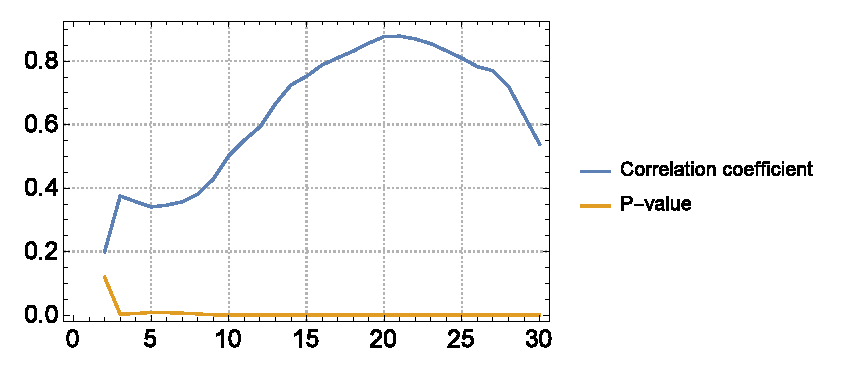
\includegraphics[width=1\linewidth]{images/A_spearman.eps}
		\subcaption{Encapsulated PostScript (.eps)}
	\end{minipage}~
	\begin{minipage}{.5\textwidth}
		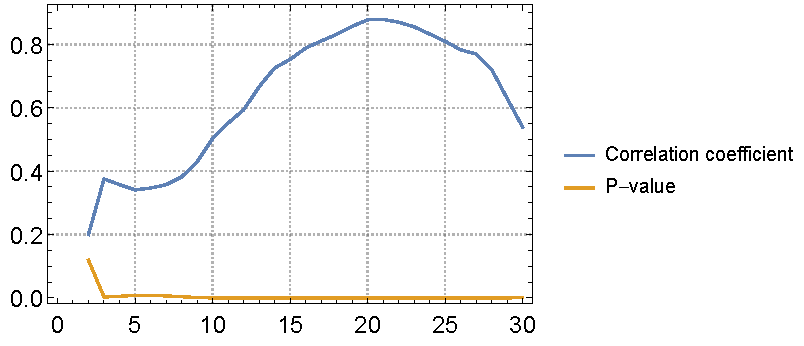
\includegraphics[width=1\linewidth]{images/A_spearman.pdf}
		\subcaption{Adobe PDF format (.pdf)}
	\end{minipage}
%	\begin{minipage}{.16\textwidth}
%		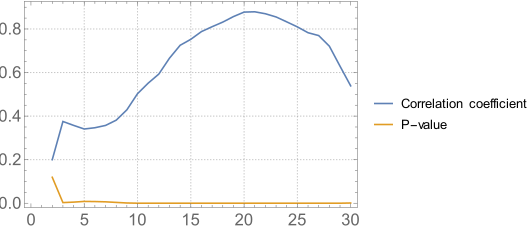
\includegraphics[width=1\linewidth]{images/A_spearman.svg}
%		\subcaption{svg}
%	\end{minipage}
	\caption{Vector graphics in 0.5 textwidth}
	\label{fig:vector_graphics}
\end{figure}

\begin{figure}
	\centering
	\begin{minipage}{.25\textwidth}
		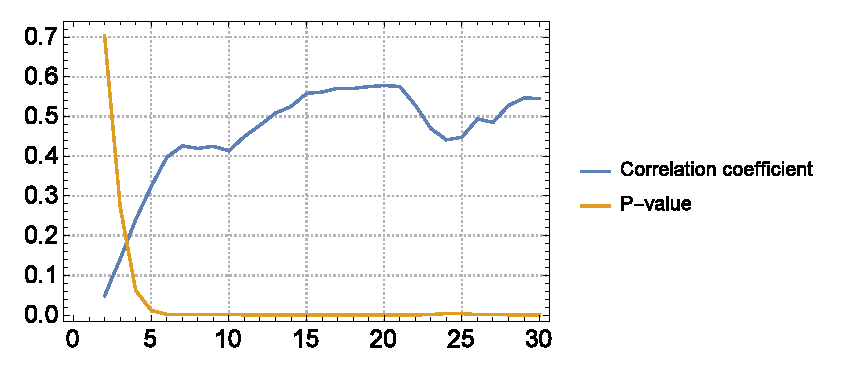
\includegraphics[width=1\linewidth]{images/B_spearman.eps}
		\subcaption{Encapsulated PostScript (.eps)}
	\end{minipage}~
	\begin{minipage}{.25\textwidth}
		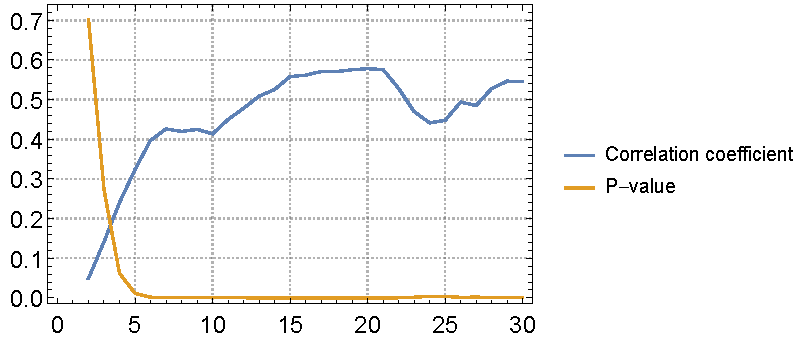
\includegraphics[width=1\linewidth]{images/B_spearman.pdf}
		\subcaption{Adobe PDF format (.pdf)}
	\end{minipage}
	%	\begin{minipage}{.16\textwidth}
	%		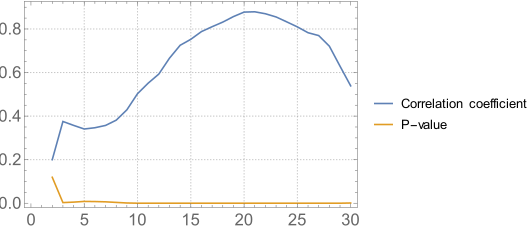
\includegraphics[width=1\linewidth]{images/A_spearman.svg}
	%		\subcaption{svg}
	%	\end{minipage}
	\caption{Vector graphics in 0.25 textwidth}
	\label{fig:vector_graphics2}
\end{figure}

\begin{figure}
	\centering
	\begin{minipage}{.125\textwidth}
		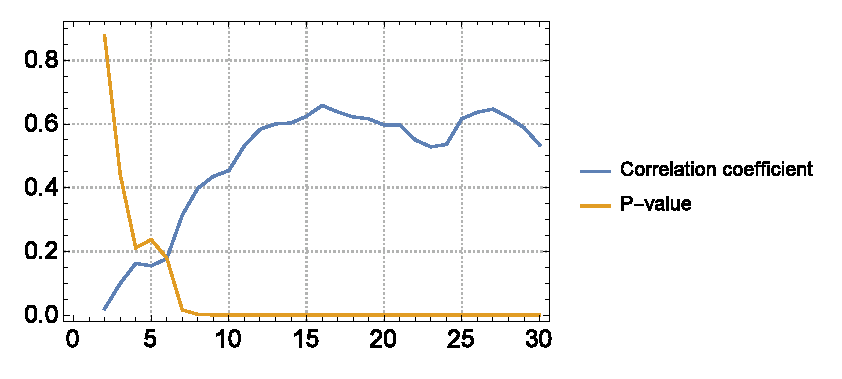
\includegraphics[width=1\linewidth]{images/C_spearman.eps}
		\subcaption{Encapsulated PostScript (.eps)}
	\end{minipage}~
	\begin{minipage}{.125\textwidth}
		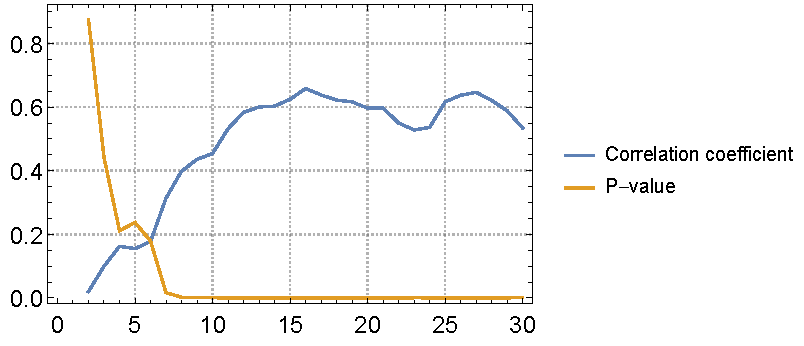
\includegraphics[width=1\linewidth]{images/C_spearman.pdf}
		\subcaption{Adobe PDF format (.pdf)}
	\end{minipage}
	%	\begin{minipage}{.16\textwidth}
	%		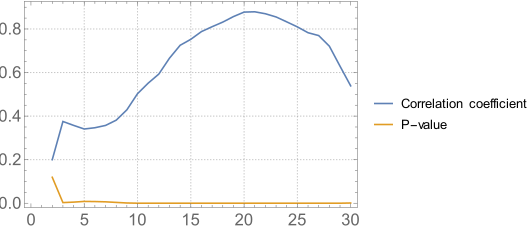
\includegraphics[width=1\linewidth]{images/A_spearman.svg}
	%		\subcaption{svg}
	%	\end{minipage}
	\caption{Vector graphics in 0.125 textwidth}
	\label{fig:vector_graphics3}
\end{figure}
	
\begin{figure}
	\centering
	\begin{minipage}{0.0625\textwidth}
		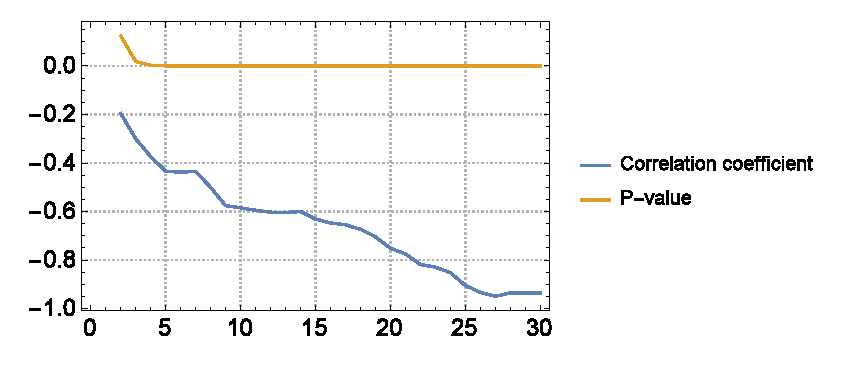
\includegraphics[width=1\linewidth]{images/D_spearman.eps}
		\subcaption{Encapsulated PostScript (.eps)}
	\end{minipage}~
	\begin{minipage}{0.0625\textwidth}
		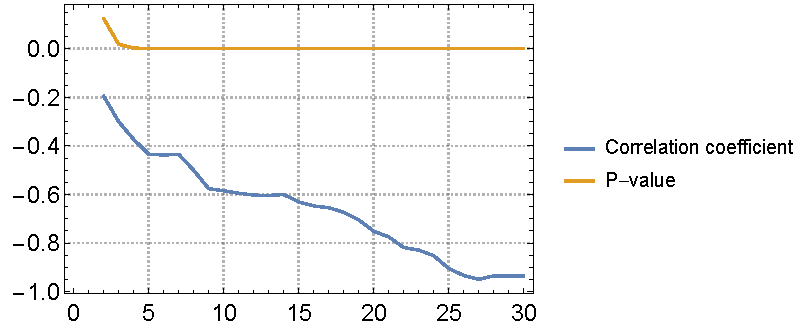
\includegraphics[width=1\linewidth]{images/D_spearman.pdf}
		\subcaption{Adobe PDF format (.pdf)}
	\end{minipage}
	%	\begin{minipage}{.16\textwidth}
	%		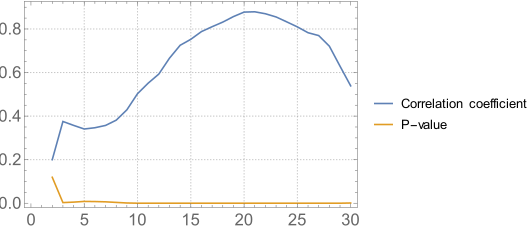
\includegraphics[width=1\linewidth]{images/A_spearman.svg}
	%		\subcaption{svg}
	%	\end{minipage}
	\caption{Vector graphics in 0.0625 textwidth}
	\label{fig:vector_graphics4}
\end{figure}
	%-------------------------------------------------------------------------
	
	%\bibliographystyle{eg-alpha}
	\bibliographystyle{eg-alpha-doi}
	
	\bibliography{egbibsample}
	
	%-------------------------------------------------------------------------

\end{document}
